Согласно структурной схеме многорежимного формирователя импульсной последовательности, данный элемент состоит из двух основных блоков:
\begin{itemize}
\item 5-разрядный счётчик
\item Фильтр импульсной последовательности
\end{itemize}

5-разрядный счётчик представляет собой готовый настраиваемый компонент САПР Quartus II - lpm\_counter. Фильтр импульсной последовательности реализуется в соответствии с функциональной схемой (см. рис. \ref{fig:secondnode}). Для реализации фильтра используются следующие элементы САПР Quartus II:
\begin{itemize}
\item элемент <<НЕ>>
\item элемент <<6-И>>
\item элемент <<2-И>>
\item элемент <<2-ИЛИ>>
\item 8-разрядный дешифратор (используются только первые шесть разрядов, см. рис. \ref{fig:dc}
\item 32-разрядный мультиплексер (используются только первые 22 разряда, см. рис. \ref{fig:mux}
\end{itemize}

\noindent Соединение элементов производится по функциональной схеме, представленной на рис. \ref{fig:secondnode}. Описание работы данной схемы представлено в разделе <<\nameref{sections:secondnode}>>.\\
Итоговая схема в САПР Quartus II представлена на рис. \ref{fig:finalscheme}.

\begin{figure}
  \begin{center}
    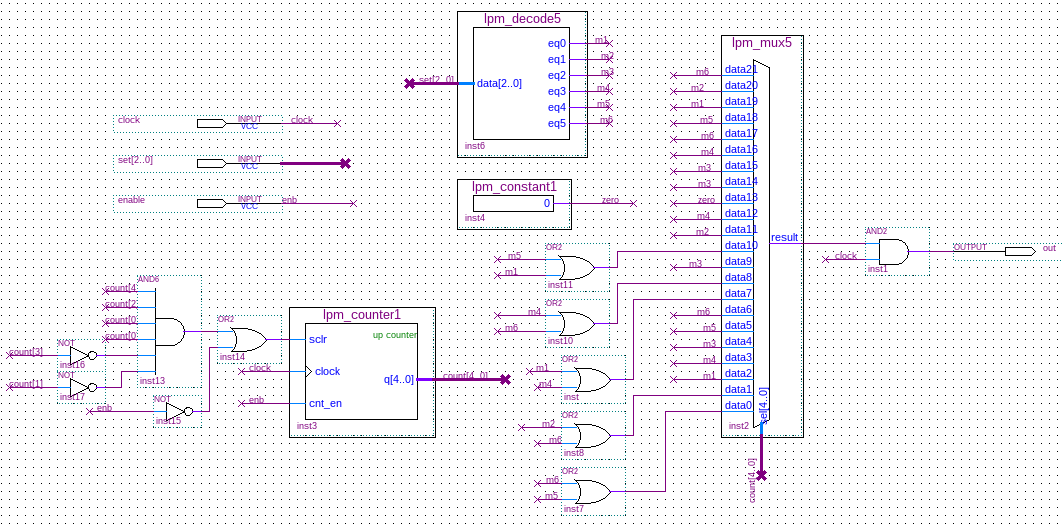
\includegraphics[scale=0.65]{./final-scheme.png}
    \caption{Итоговая схема в САПР Quartus II.}
    \label{fig:finalscheme}
  \end{center}
\end{figure}